\documentclass[12pt,a4paper,twoside]{article}
    \special{papersize=210mm,297mm}
    
    \usepackage[a4paper,includeheadfoot,margin=2.54cm]{geometry}
    \usepackage{pdflscape}
    \usepackage{hyperref}
    \usepackage{natbib}
    \usepackage{cmbright}
    \usepackage[utf8]{inputenc}
    \usepackage{graphicx}
    \usepackage[english,danish]{babel}

    \usepackage[familydefault,regular]{Chivo}
    \usepackage[T1]{fontenc}

    \usepackage{lastpage}
    \usepackage{fancyhdr}
    \usepackage[usenames,dvipsnames,svgnames,table]{xcolor}
    \usepackage{mathtools}
    \usepackage{amsmath}
    \usepackage{gensymb}
    %Plotning af 
    \usepackage{pgfplots}
    \usepackage{pdfpages}
    %\pgfplotset{width=10cm,compat=1.9}
    \usepackage{multirow}     
    %\usepackage{tabularx}
    \usepackage{booktabs}% http://ctan.org/pkg/booktabs
                  
    \pagestyle{fancy} 
    \fancyhf{}
    \fancyhead[LE,RO]{Power Supply Unit}
    \fancyhead[RE,LO]{\rightmark}
    \fancyfoot[CE,CO]{Michael Torp Kaalund}
    \fancyfoot[LE,RO]{Side \thepage \hspace{1pt} af \pageref{LastPage}}
    \renewcommand{\headrulewidth}{1.5pt}
    \renewcommand{\footrulewidth}{1.5pt}
 
    %% Ny 
    \newcommand{\vdc}{V$_{\text{DC}}$ }
    \newcommand{\vac}{V$_{\text{AC}}$ }
    \newcommand{\tabitem}{~~\llap{\textbullet}~~}
    \newcommand{\todo}[1]{\textcolor{red}{TODO: #1}\PackageWarning{TODO:}{#1!}}

    \title{Power Supply Unit}
    
    \author{Michael Torp Kaalund}

\begin{document}
\selectlanguage{english}
\begin{titlepage}
    \centering
    {\usefont{T1}{pag}{m}{b}\LARGE Power Supply Unit \par}
    \vspace{1cm}
    \vspace{1cm}
    {\usefont{T1}{fvs}{m}{b}\Large First iteration of PSU \par}
    \vspace{1.5cm}
    {\huge\bfseries Version 1 \par}
    \vspace{10cm}
    {\usefont{T1}{qzc}{m}{it} Michael Torp Kaalund \par}
    \vfill
    {\bfseries \today\par}
\end{titlepage}
\newpage
\tableofcontents

\section{Design \& Calculations}
In this section we will calculate the required values of our input circuit,
and our regular design.
\section{Input Circuit}
In Europe the mains voltage in houses is 230 volts, all of the input circuit before the transformer needs to be designed to that voltages. 
As this part of the input circuit we want to besure that the noise on mains volts do not propegate to our output volts, we are going to use a $\pi$-filter to filter out some noise. This will also double as filter for any noise we are going to send out to the mains voltage. The one I am going to use is one that I have bougth a long time ago. As a means for input protection we are also going to use fuse (see formula \ref{eq:transfer-transformer} on page \pageref{eq:transfer-transformer}).

\subsection{Transformer}
The transfer formula for the transformer 
\begin{align}\label{eq:transfer-transformer}
m &= \frac{I_s}{I_p} = \frac{V_p}{V_s}
\end{align}
For the input supply I am going to use a transformer 2x18V at 1.5A, that I already have. And I am going to connect the 18V's in series to get 36V at 1.5A. But for finding the transfer value we can use formula \ref{eq:transfer-transformer}.
\begin{align}
m = \frac{V_p}{V_s} = \frac{230V}{18V} = 12.78 \nonumber
\end{align}
 To find out which size of fuse that we are going to be using, we need to find out how much current that are going to be used on the main side of the transformer.
We are going rearrange in formula \ref{eq:transfer-transformer} as we know what $I_s$ is and we have calculated $m$.
\begin{align}
m = \frac{I_s}{I_p} \nonumber \\
\Rightarrow \nonumber \\
I_p \cdot m = I_p \cdot \frac{I_s}{I_p} = I_s \nonumber \\
\Rightarrow \nonumber \\
\frac{ I_p \cdot m}{m} = \frac{I_s}{m} \nonumber \\
\Rightarrow \nonumber \\
I_p = \frac{I_s}{m} \label{eq:found-Ip}
\end{align}
Now we can calculate $I_p$ with $I_s$ and $m$ from \ref{eq:found-Ip}.
\begin{align}
I_p = \frac{I_s}{m} = \frac{1.5A}{12.78} = 0.117A = \underline{\underline{117mA}} \nonumber 
\end{align}
So the primary side of the transformer needs a fuse of 117mA, but as I can not find that size, the one that is going to be used is a 125mA.

The 36 volt ac are going to be converted to dc, via fullwave diode bridge. Sinces the ac voltage specified on the transformer is RMS voltage, an not the peak voltage. We can calculate what the dc voltage will become assuming no losses.
\begin{align} \label{eq:calc_vdc}
V_{ dc } &= \frac{ 2 \cdot V_{ max } }{ \pi } \\
         &= 0.637 \cdot V_{ max } \\
         &= 0.9 \cdot V_{ RMS } \\
         &= 0.9 \cdot 36 V_{ac} \nonumber \\
         &= 32.4 V_{ dc } \nonumber
\end{align}
But since we are going to use a bridge rectifier there is two times diode voltage drop that gives total drop of \(1.4V\). Which meaning that we are properly only going to see around \( 31V \) if measure at the diode bridge output. And the 50Hz frequency is being doubled to 100Hz.

\subsection{Ripple voltage}

\begin{align}\label{eq:calc_vripple}
V_{ ripple } &= \frac{ I_{ load } }{ f \times C } [V]
\end{align}
 
\section{Regulator}

We will be using a LM317 for the current and voltage regulations, 
as this is a cheap regulator and it is well known. 
This design will also have a 5V supply, 
which can be created from a LM7805 or with a LM317 with two resistors.

\subsection{Current Regulator}
In the datasheet of the LM317, there is a referece on how use it in a current limiting capacity as seen on figure \ref{fig:lm317_current_limit}.
\begin{figure}[ht]
    \centering
    \caption{LM317 Current-Limiter Circuit}\label{fig:lm317_current_limit}
    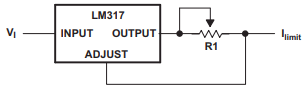
\includegraphics{img/current_limit.png}
\end{figure}

Here the current output will be 
\begin{align}
    \text{I}_{limit} &= \frac{\text{V}_{\text{ref}}}{R_{1}} \label{eq:i_limit_lm317}
\end{align}

The V$_{\text{ref}}$ is between 1.2 V and 1.3 V, and typically it is 1.25 V which is what we are going to use for calculations.
If we rearrance formula \ref{eq:i_limit_lm317} so we get $R_{1}$.
\begin{align}
    \text{I}_{limit} \cdot R_{1} &= R_{1} \cdot \frac{\text{V}_{\text{ref}}}{R_{1}} \nonumber \\
    \Downarrow  \nonumber \\
    \text{I}_{limit} \cdot R_{1} &= \text{V}_{\text{ref}} \nonumber \\
    \Downarrow  \nonumber \\
    \frac{ \text{I}_{limit} \cdot R_{1} }{\text{I}_{limit}} &= \frac{\text{V}_{\text{ref}}}{\text{I}_{limit}} \nonumber \\
    \Downarrow  \nonumber \\
    R_{1} &= \frac{\text{V}_{\text{ref}}}{\text{I}_{limit}}\\
\end{align}
So now we can calculate for the maximum current
\begin{align}
    R_{1}   &= \frac{\text{V}_{\text{ref}}}{\text{I}_{limit}} \nonumber \\
            &= \frac{1.25 \text{V}}{1.5\text{A}} \nonumber \\
            &= \underline{ \underline{ 0.8333 \Omega}}
\end{align}
As the closes resistor we can get is 0.82 $\Omega$ this is the one we are going to choose.
The next we want to calculate is the paralle resistor, this is the one which can be adjusted.

\section{Prototyping}

\appendix

\chapter{SI-Prefix}

\[
\begin{array}{|c|c|c|}
\firsthline
Name    & Symbol & 10^{n}  \\
\hline
\hline
yotta 	& Y	& 10^{24}	 \\ \hline
zetta	& Z	& 10^{21}	 \\ \hline
exa	& E	& 10^{18}	 \\ \hline
peta	& P	& 10^{15}	 \\ \hline
tera	& T	& 10^{12}	 \\ \hline
giga	& G	& 10^{9}	 \\ \hline
mega	& M	& 10^{6}	 \\ \hline
kilo	& k	& 10^{3}	 \\ \hline
hecto	& h	& 10^{2}	 \\ \hline
deca	& da	& 10^{1}	 \\ \hline
	&    	& 10^{0}	 \\ \hline
deci	& d  	& 10^{-1}	 \\ \hline
centi	& c  	& 10^{-2}	 \\ \hline
milli	& m  	& 10^{-3}	 \\ \hline
micro	& \mu 	& 10^{-6}	 \\ \hline
nano	& n	& 10^{-9} 	 \\ \hline
pico	& p	& 10^{-12}	 \\ \hline
femto	& f	& 10^{-15}	 \\ \hline
atto	& a	& 10^{-18}	 \\ \hline
zepto	& z	& 10^{-21}	 \\ \hline
yocto	& y	& 10^{-24}	 \\ \hline
\end{array}
\]

\section{Bill Of Materials}

\begin{tabular}[c]{|l|l|l|r|c|r|}
\hline
 & Store & Description & Price a piece & QTY & Total price \\
 \hline
 & \url{www.aliexpress.com} & 3-pin Panel mount filter EMI 115 / 8A 220 V AC 50/60Hz Power Filter BALnector & US\$1.77 & 1 & US\$1.77 \\
 & \url{www.aliexpress.com} & 30W double 18V 30W2*18V transformer, power transformer input, 220V, 50Hz/ output, double 18V & US\$6.66(+ shipping US\$8.76) & 1 & US\$15.42 \\
 & \url{www.aliexpress.com} & 10PC/Lot New 2W10 2A 1000V Diode Bridge Rectifier replace 2W06 2W08 & US\$0.89 & 1 & US\$0.89 \\
\hline
\end{tabular}

\end{document}
